% Standalone Fig. 1 - 可在 TikZMaker (https://tikzmaker.com) 中直接编辑
% 也可用 pdflatex fig1_standalone.tex 独立编译
\documentclass[border=5pt]{standalone}
\usepackage{amsmath,amssymb}
\usepackage{tikz}
\usepackage{pifont}
\usetikzlibrary{
  positioning, arrows.meta, shapes.geometric, shapes.multipart,
  fit, backgrounds, calc, decorations.pathreplacing, patterns,
  shadows.blur, chains
}

% Color definitions (same as main.tex)
\definecolor{inputblue}{HTML}{D6EAF8}
\definecolor{inputborder}{HTML}{2E86C1}
\definecolor{plannerorg}{HTML}{FDEBD0}
\definecolor{plannerborder}{HTML}{E67E22}
\definecolor{memgreen}{HTML}{D5F5E3}
\definecolor{memborder}{HTML}{27AE60}
\definecolor{execpink}{HTML}{FADBD8}
\definecolor{execborder}{HTML}{E74C3C}
\definecolor{skillblue}{HTML}{D4E6F1}
\definecolor{skillborder}{HTML}{2980B9}
\definecolor{arrowred}{HTML}{C0392B}
\definecolor{arrowgreen}{HTML}{27AE60}
\definecolor{arrowblue}{HTML}{2E86C1}
\definecolor{arrowgray}{HTML}{7F8C8D}
\definecolor{reflectpurple}{HTML}{8E44AD}
\definecolor{l1gold}{HTML}{F39C12}

\begin{document}
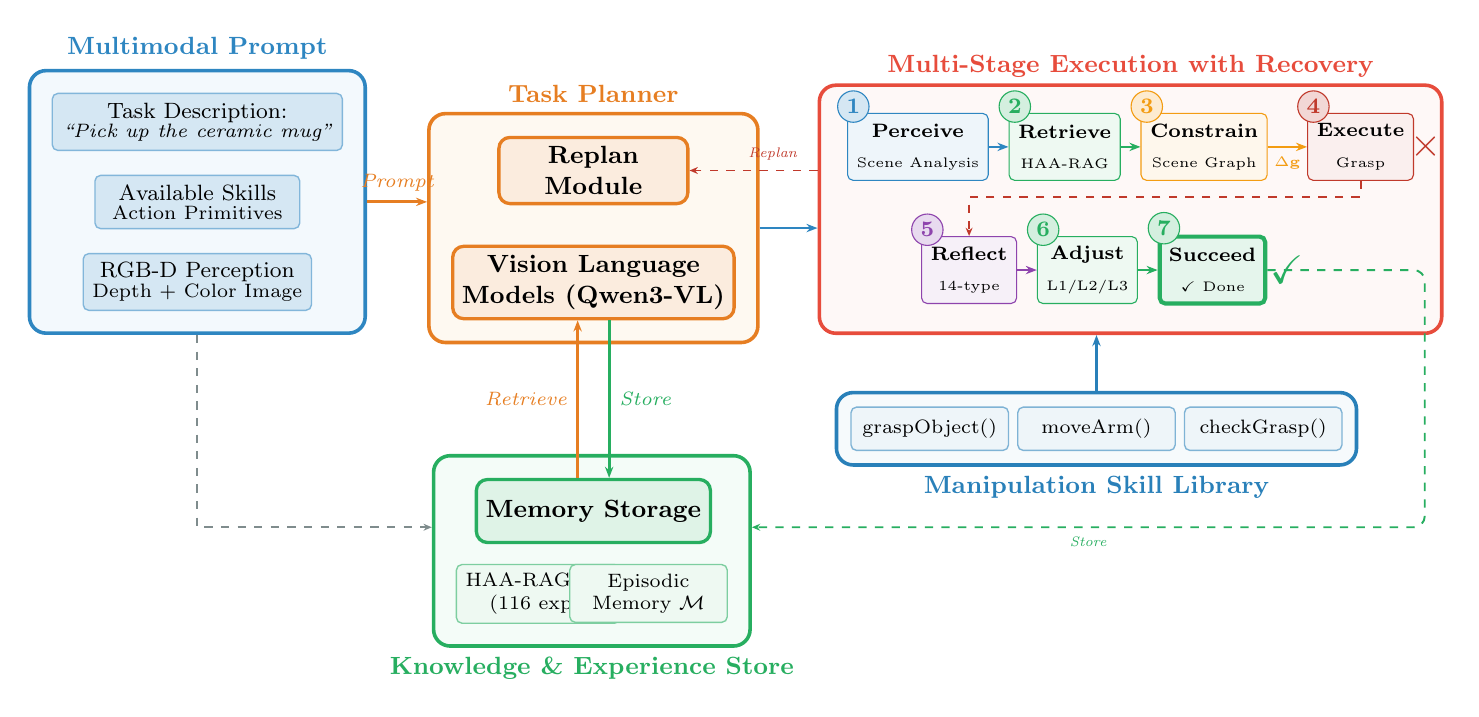
\begin{tikzpicture}[
  >=Stealth,
  node distance=0.4cm and 0.5cm,
  mainblock/.style={
    rectangle, rounded corners=4pt,
    draw=#1, fill=#1!15, line width=1.2pt,
    minimum width=2.4cm, minimum height=0.8cm,
    font=\small\bfseries, text=black, align=center
  },
  subblock/.style={
    rectangle, rounded corners=2pt,
    draw=#1!60, fill=#1!8, line width=0.5pt,
    minimum width=2cm, minimum height=0.45cm,
    font=\scriptsize, text=black, align=center
  },
  ioblock/.style={
    rectangle, rounded corners=2pt,
    draw=#1!60, fill=#1!20, line width=0.5pt,
    minimum height=0.5cm,
    font=\scriptsize, text=black, align=center
  },
  groupbox/.style 2 args={
    rectangle, rounded corners=6pt,
    draw=#1, fill=#2, line width=1.3pt,
    inner sep=8pt
  },
  grouplabel/.style={
    font=\small\bfseries, text=#1
  },
  myarrow/.style={
    ->, line width=1pt, color=#1,
    >={Stealth[length=4pt, width=3pt]}
  },
  dashedarrow/.style={
    ->, line width=0.7pt, dashed, color=#1,
    >={Stealth[length=3pt, width=2.5pt]}
  },
  steplabel/.style={
    circle, draw=#1, fill=#1!20,
    inner sep=1.5pt, font=\scriptsize\bfseries, text=#1
  }
]
% === LEFT: Multimodal Prompt ===
\node[ioblock=inputborder, minimum width=2.6cm, minimum height=0.55cm] (taskdesc)
  {\footnotesize Task Description:\\[-1pt]\scriptsize\itshape ``Pick up the ceramic mug''};
\node[ioblock=inputborder, minimum width=2.6cm, below=0.3cm of taskdesc] (skilllist)
  {\footnotesize Available Skills\\[-1pt]\scriptsize Action Primitives};
\node[ioblock=inputborder, minimum width=2.6cm, below=0.3cm of skilllist] (rgbd)
  {\footnotesize RGB-D Perception\\[-1pt]\scriptsize Depth + Color Image};
\begin{scope}[on background layer]
  \node[groupbox={inputborder}{inputblue!30}, fit=(taskdesc)(skilllist)(rgbd),
      label={[grouplabel=inputborder]above:Multimodal Prompt}] (inputbox) {};
\end{scope}

% === CENTER: Task Planner ===
\node[mainblock=plannerborder, right=2.5cm of skilllist, yshift=0.4cm] (replan)
  {Replan\\Module};
\node[mainblock=plannerborder, below=0.5cm of replan] (vlm)
  {Vision Language\\Models (Qwen3-VL)};
\begin{scope}[on background layer]
  \node[groupbox={plannerborder}{plannerorg!30}, fit=(replan)(vlm),
      label={[grouplabel=plannerborder]above:Task Planner}] (plannerbox) {};
\end{scope}

% === BOTTOM CENTER: Memory Storage ===
\node[mainblock=memborder, below=2cm of vlm] (memory)
  {Memory Storage};
\node[subblock=memborder, below=0.25cm of memory, xshift=-0.7cm] (chromadb)
  {HAA-RAG KB\\(116 exp.)};
\node[subblock=memborder, below=0.25cm of memory, xshift=0.7cm] (episodic)
  {Episodic\\Memory $\mathcal{M}$};
\begin{scope}[on background layer]
  \node[groupbox={memborder}{memgreen!25}, fit=(memory)(chromadb)(episodic),
      label={[grouplabel=memborder]below:Knowledge \& Experience Store}] (membox) {};
\end{scope}

% === RIGHT: Multi-Stage Execution ===
\node[rectangle, draw=arrowblue, fill=arrowblue!8, minimum width=1.05cm, minimum height=0.85cm,
  rounded corners=2pt, align=center, right=2cm of replan, yshift=0.3cm] (step1)
  {\scriptsize\textbf{Perceive}\\[-1pt]\tiny Scene Analysis};
\node[rectangle, draw=memborder, fill=memborder!8, minimum width=1.05cm, minimum height=0.85cm,
  rounded corners=2pt, align=center, right=0.25cm of step1] (step2)
  {\scriptsize\textbf{Retrieve}\\[-1pt]\tiny HAA-RAG};
\node[rectangle, draw=l1gold, fill=l1gold!8, minimum width=1.05cm, minimum height=0.85cm,
  rounded corners=2pt, align=center, right=0.25cm of step2] (step3)
  {\scriptsize\textbf{Constrain}\\[-1pt]\tiny Scene Graph};
\node[rectangle, draw=arrowred, fill=arrowred!8, minimum width=1.05cm, minimum height=0.85cm,
  rounded corners=2pt, align=center, right=0.5cm of step3] (step4)
  {\scriptsize\textbf{Execute}\\[-1pt]\tiny Grasp};
\node[steplabel=arrowblue] at ($(step1.north west)+(0.08,0.08)$) {\footnotesize 1};
\node[steplabel=memborder] at ($(step2.north west)+(0.08,0.08)$) {\footnotesize 2};
\node[steplabel=l1gold] at ($(step3.north west)+(0.08,0.08)$) {\footnotesize 3};
\node[steplabel=arrowred] at ($(step4.north west)+(0.08,0.08)$) {\footnotesize 4};
\node[font=\Large, text=arrowred] at ($(step4.east)+(0.15,0)$) {$\times$};

% Recovery row
\node[rectangle, draw=reflectpurple, fill=reflectpurple!8, minimum width=1.05cm, minimum height=0.85cm,
  rounded corners=2pt, align=center, below=0.7cm of step1, xshift=0.65cm] (step5)
  {\scriptsize\textbf{Reflect}\\[-1pt]\tiny 14-type};
\node[rectangle, draw=arrowgreen, fill=arrowgreen!8, minimum width=1.05cm, minimum height=0.85cm,
  rounded corners=2pt, align=center, right=0.25cm of step5] (step6)
  {\scriptsize\textbf{Adjust}\\[-1pt]\tiny L1/L2/L3};
\node[rectangle, draw=arrowgreen, fill=arrowgreen!12, minimum width=1.05cm, minimum height=0.85cm,
  rounded corners=2pt, align=center, line width=1.5pt, right=0.25cm of step6] (step7)
  {\scriptsize\textbf{Succeed}\\[-1pt]\tiny $\checkmark$ Done};
\node[steplabel=reflectpurple] at ($(step5.north west)+(0.08,0.08)$) {\footnotesize 5};
\node[steplabel=arrowgreen] at ($(step6.north west)+(0.08,0.08)$) {\footnotesize 6};
\node[steplabel=arrowgreen] at ($(step7.north west)+(0.08,0.08)$) {\footnotesize 7};
\node[font=\Large, text=arrowgreen] at ($(step7.east)+(0.25,0)$) {\checkmark};
\begin{scope}[on background layer]
  \node[groupbox={execborder}{execpink!20}, fit=(step1)(step2)(step3)(step4)(step5)(step6)(step7),
    inner sep=10pt,
    label={[grouplabel=execborder, fill=white, inner sep=2pt]above:Multi-Stage Execution with Recovery}] (execbox) {};
\end{scope}

% Execution arrows
\draw[myarrow=arrowblue] (step1) -- (step2);
\draw[myarrow=memborder] (step2) -- (step3);
\draw[myarrow=l1gold] (step3) -- (step4)
  node[midway, below, font=\tiny\bfseries, text=l1gold] {$\Delta\mathbf{g}$};
\draw[dashedarrow=arrowred] (step4.south) -- ++(0, -0.2) -| (step5.north);
\draw[myarrow=reflectpurple] (step5) -- (step6);
\draw[myarrow=arrowgreen] (step6) -- (step7);

% === BOTTOM RIGHT: Skill Library ===
\node[subblock=skillborder, minimum height=0.55cm, below=1.3cm of step5, xshift=-0.5cm] (sk1) {graspObject()};
\node[subblock=skillborder, minimum height=0.55cm, right=0.1cm of sk1] (sk2) {moveArm()};
\node[subblock=skillborder, minimum height=0.55cm, right=0.1cm of sk2] (sk3) {checkGrasp()};
\begin{scope}[on background layer]
  \node[groupbox={skillborder}{skillblue!20}, fit=(sk1)(sk2)(sk3), inner sep=5pt,
    label={[grouplabel=skillborder]below:Manipulation Skill Library}] (skillbox) {};
\end{scope}

% === MAIN ARROWS ===
% Prompt: horizontal from input to planner
\draw[myarrow=plannerborder] (inputbox.east) -- (plannerbox.west |- inputbox.east)
  node[midway, above, font=\scriptsize\itshape, text=plannerborder] {Prompt};
% Blue arrow: horizontal from planner to exec
\draw[myarrow=arrowblue] (plannerbox.east) -- (execbox.west |- plannerbox.east);
% Store / Retrieve between VLM and Memory
\draw[myarrow=memborder] ($(vlm.south)+(0.2, 0)$) -- ($(memory.north)+(0.2, 0)$)
  node[midway, right, font=\scriptsize\itshape, text=memborder] {Store};
\draw[myarrow=plannerborder] ($(memory.north)+(-0.2, 0)$) -- ($(vlm.south)+(-0.2, 0)$)
  node[midway, left, font=\scriptsize\itshape, text=plannerborder] {Retrieve};
% Gray dashed: from inputbox bottom (avoid passing through blue box)
\draw[dashedarrow=arrowgray] (inputbox.south) |- ($(membox.west)+(0, 0.3)$);
% Green Store: from Succeed right side, route around skill library
\draw[dashedarrow=arrowgreen, rounded corners=4pt]
  (step7.east) -- ++(2.0, 0) |- ($(membox.east)+(0, 0.3)$)
  node[near end, below, font=\tiny\itshape, text=arrowgreen] {Store};
% Skill library to exec: vertical
\draw[myarrow=skillborder] (skillbox.north) -- (skillbox.north |- execbox.south);
% Replan: horizontal only from exec left edge to replan
\draw[dashedarrow=arrowred] (execbox.west |- replan.east) -- (replan.east)
  node[pos=0.35, above, font=\tiny\itshape, text=arrowred] {Replan};
\end{tikzpicture}
\end{document}
